\documentclass[11pt]{article}

\usepackage[margin=1in]{geometry}
% Compile this document with XeLaTeX to preserve Vietnamese examples.
\usepackage{fontspec}
\setmainfont{Arial}
\usepackage{microtype}
\usepackage{amsmath}
\usepackage{booktabs}
\usepackage{tabularx}
\usepackage{graphicx}
\usepackage{caption}
\usepackage{enumitem}
\usepackage[hidelinks]{hyperref}
\usepackage[numbers,sort&compress]{natbib}

\setlength{\parindent}{1.5em}
\setlength{\parskip}{0.25em}
\setlength{\emergencystretch}{2em}
\setlist[itemize]{noitemsep,topsep=0pt}
\renewcommand{\arraystretch}{1.15}

\begin{document}
\begin{titlepage}
\thispagestyle{empty}
\begin{center}
{\large \textbf{UNIVERSITY:} \rule{8cm}{0.4pt}}\\[1em]
{\large \textbf{FACULTY / DEPARTMENT:} \rule{6cm}{0.4pt}}\\[3em]
{\Large \textbf{FINAL PROJECT REPORT}}\\[2em]
{\LARGE \textbf{Vietnamese Social Media Lexical Normalization with BARTpho}}\\[1em]
{\large A Comparative Study of Gold and LLM-Reviewed Weak-Label Training}\\[3em]
\begin{tabular}{ll}
\textbf{Course:} & Statistical Learning \\[1em]
\textbf{Instructor:} & \rule{8cm}{0.4pt} \\[2em]
\textbf{Student 1:} & \rule{5cm}{0.4pt}\quad \textbf{ID:} \rule{3cm}{0.4pt} \\[1em]
\textbf{Student 2:} & \rule{5cm}{0.4pt}\quad \textbf{ID:} \rule{3cm}{0.4pt} \\[1em]
\textbf{Student 3:} & \rule{5cm}{0.4pt}\quad \textbf{ID:} \rule{3cm}{0.4pt} \\[1em]
\textbf{Student 4:} & \rule{5cm}{0.4pt}\quad \textbf{ID:} \rule{3cm}{0.4pt}
\end{tabular}
\vfill
\textbf{Submission date:} \rule{5cm}{0.4pt}
\end{center}
\end{titlepage}
\setcounter{page}{1}

\begin{abstract}
Vietnamese social media text frequently contains abbreviations, informal spellings, omitted diacritics, and other non-standard lexical forms. This study formulates their normalization as a sequence-to-sequence task and compares three BARTpho-syllable configurations. Model~A was fine-tuned on 8,372 human-annotated ViLexNorm training pairs. Model~B was initialized from Model~A and trained with a balanced mixture of gold data and an initial pool of 18,970 LLM-reviewed weak labels. Model~C was also initialized from Model~A but used an expanded pool of 64,813 LLM-reviewed weak labels. Candidate normalizations for ViSoLex were reviewed by Gemini under a \textsc{Keep}, \textsc{Edit}, or \textsc{Reject} protocol and then subjected to deterministic validation. A common Dev evaluation selected Model~C before final Test scoring. On the 1,045-sentence ViLexNorm Test split, Models~A, B, and C obtained F1 scores of 0.7182, 0.7422, and 0.7650, and Error Reduction Rates of 0.6002, 0.6331, and 0.6647, respectively. Model~C was used for a local Gradio application, with Model~B retained as a fallback checkpoint. The application performs BARTpho inference locally and does not use the review model at runtime.
\end{abstract}

\section{Introduction}

Vietnamese social media messages often depart from conventional written forms. Users may shorten words, omit diacritics, write phonetic variants, or use informal lexical forms that are understandable in context but difficult for downstream language-processing systems to interpret consistently. For example, the sentence \textit{mik ko bt hnay đi hc ko} can be normalized as \textit{mình không biết hôm nay đi học không}. This transformation changes lexical forms such as \textit{mik}, \textit{ko}, \textit{bt}, \textit{hnay}, and \textit{hc}, while preserving the intended proposition and the overall sentence structure.

The present work treats this problem as lexical normalization rather than unrestricted rewriting. The intended output is a more canonical lexical realization of the input, not a paraphrase, a stylistic reformulation, a full grammatical correction, or an alteration of sentiment and content. This distinction matters because a system that rewrites a sentence fluently may still be unsuitable for lexical normalization if it changes information that was not expressed in the source text.

The available supervised resource, ViLexNorm, provides human-annotated pairs of noisy and normalized Vietnamese social media sentences \citep{nguyen2024vilexnorm}. Its 8,372-example training split provides a direct basis for supervised fine-tuning, but social media language is diverse and its lexical variation is not fully represented by a moderate-sized gold corpus. In contrast, the processed ViSoLex corpus used in this project contains 68,411 unlabeled social media sentences. The central question of this study is therefore whether LLM-reviewed labels constructed from this unlabeled corpus can provide additional training signal for a BARTpho model.

The study compares three configurations of the same BARTpho-syllable architecture. Model~A uses only ViLexNorm gold training data. Model~B continues from Model~A with an initial LLM-reviewed weak-label pool of 18,970 examples. Model~C also continues from Model~A but uses an expanded LLM-reviewed weak-label pool of 64,813 examples. The comparison is designed to examine how the composition and coverage of LLM-reviewed weak-label data are associated with lexical-normalization performance. The project further implements a local Gradio application using the model selected on Dev, so that inference does not require the training corpus or an external review API.

\section{Background and Related Work}

\subsection{Lexical normalization}

Lexical normalization maps non-standard lexical forms to conventional or canonical forms. The mapping may be one-to-one, as in an abbreviation expanded to one standard word, but it may also be one-to-many or many-to-one. A short form such as \textit{đky} may become \textit{đăng ký}, whereas other transformations may merge or reorder whitespace-delimited units. Consequently, the task is naturally expressed as conditional sequence generation rather than as a collection of independent token classifications.

ViLexNorm introduced a Vietnamese lexical-normalization corpus containing more than 10,000 human-annotated sentence pairs collected from public social media comments \citep{nguyen2024vilexnorm}. The source study evaluated systems with Error Reduction Rate (ERR) relative to a Leave-As-Is baseline and reported a BARTpho-syllable result of 57.74\% under its evaluation setting. The project reported here uses the ViLexNorm Train, Dev, and Test splits as supplied, but it implements a deterministic token-edit scorer because the referenced corpus repository distributes data rather than an official evaluator. Its numerical results should therefore be interpreted within the project evaluation protocol rather than compared directly with values reported by another implementation.

\subsection{From Transformer to BARTpho}

The Transformer introduced an encoder--decoder architecture that relies on attention rather than recurrence or convolution \citep{vaswani2017attention}. In an encoder--decoder setting, the encoder constructs contextual representations of the input sequence, while the decoder produces output tokens autoregressively. Self-attention allows each token representation to use information from other positions in the same sequence. In its standard scaled dot-product form, attention is written as
\begin{equation}
\operatorname{Attention}(Q,K,V)=
\operatorname{softmax}\left(\frac{QK^{\mathsf{T}}}{\sqrt{d_k}}\right)V,
\end{equation}
where $Q$, $K$, and $V$ denote query, key, and value projections. The weighting operation determines how strongly each position uses information from other positions. Multi-head attention applies several such projections in parallel.

BART is a denoising sequence-to-sequence model. During pre-training, its input text is corrupted and the model learns to reconstruct the original text \citep{lewis2020bart}. This objective does not directly train social media lexical normalization, but it provides an encoder--decoder initialization for conditional reconstruction. The generated sequence may differ in length from the source sequence, which is useful when a non-standard social media form must be expanded or contracted.

BARTpho adapts the BART sequence-to-sequence approach to Vietnamese \citep{tran2022bartpho}. It provides word-level and syllable-level variants and is based on the BART-large architecture. This project uses \texttt{vinai/bartpho-syllable}. The syllable-level variant is appropriate for the present preprocessing pipeline because noisy forms such as \textit{mik}, \textit{hnay}, and \textit{khum} do not require a separate Vietnamese word-segmentation step before they are passed to the model. This choice does not imply that the syllable-level variant is universally preferable; it matches the lexical characteristics and input representation of the current task.

\section{Task Formulation and Experimental Design}

Let $x=(x_1,\ldots,x_m)$ denote a noisy social media sentence and let $y=(y_1,\ldots,y_n)$ denote its normalized form. A sequence-to-sequence model with parameters $\theta$ estimates the conditional probability
\begin{equation}
P(y\mid x;\theta)=\prod_{t=1}^{n}P(y_t\mid y_{<t},x;\theta).
\end{equation}
The output length $n$ need not equal the input length $m$. This property permits the model to represent one-to-many and many-to-one lexical mappings without adding a separate alignment module.

The experimental variable is the reviewed weak-label data available during training. Model~A receives only human-annotated ViLexNorm pairs. Models~B and C are initialized from Model~A and receive balanced mixtures of the same gold training data with reviewed ViSoLex weak labels. Model~B uses the initial accepted pool, whereas Model~C uses the expanded accepted pool. The three configurations share the same BARTpho-syllable architecture, tokenizer family, maximum sequence lengths, decoding configuration, and validation set.

The comparison should not be read as a perfect isolation of weak-label count. Model~A begins from the public BARTpho checkpoint, whereas Models~B and C continue from Model~A. Models~B and C also use different training durations because their weak-label pools have different sizes. The results consequently compare complete training configurations: initial checkpoint, data composition, sampling schedule, and number of epochs. This qualification is retained throughout the analysis.

\begin{figure}[t]
\centering
\fbox{\parbox{0.91\linewidth}{\centering\small
\vspace{0.45em}
\textbf{Shared architecture:} BARTpho-syllable\\[0.6em]
\begin{tabular}{@{}>{\raggedright\arraybackslash}p{0.27\linewidth}@{\hspace{0.02\linewidth}}>{\raggedright\arraybackslash}p{0.27\linewidth}@{\hspace{0.02\linewidth}}>{\raggedright\arraybackslash}p{0.27\linewidth}@{}}
\textbf{Model A} & \textbf{Model B} & \textbf{Model C}\\
Gold-only training & Gold + initial reviewed pool & Gold + expanded reviewed pool\\
8,372 gold pairs & 8,372 gold pairs + 18,970 weak labels & 8,372 gold pairs + 64,813 weak labels
\end{tabular}\\[0.6em]
Model~A also provides the candidate-generation and initialization provenance for Models~B and C.
\vspace{0.45em}}}
\caption{Three BARTpho-syllable training configurations. The visual layout presents the configurations symmetrically, while the final sentence records their actual checkpoint provenance.}
\label{fig:configurations}
\end{figure}

\section{Data Preparation and Weak-Label Construction}

\subsection{Gold data and unlabeled corpus}

ViLexNorm was retained in its original Train, Dev, and Test partitioning. The training split contains 8,372 examples, the development split contains 1,050 examples, and the test split contains 1,045 examples. Each processed record stores an identifier, dataset name, split name, noisy input, normalized target, and the label source. Preprocessing normalizes whitespace and removes records with empty input or target fields, but it does not correct lexical noise before training. Retaining noise is necessary because the noise itself constitutes the input signal for normalization.

\begin{table}[t]
\centering
\caption{ViLexNorm splits used by the project.}
\label{tab:vilexnorm-splits}
\begin{tabular}{lrl}
\toprule
Split & Examples & Use \\
\midrule
Train & 8,372 & Fine-tuning \\
Dev & 1,050 & Checkpoint selection and development analysis \\
Test & 1,045 & Comparative evaluation \\
\bottomrule
\end{tabular}
\end{table}

The additional unlabeled corpus follows the source composition released with ViSoLex \citep{nguyen2025visolex}. The initial specification expected approximately 121,087 sentences; this is a planning estimate, not an observed raw count for the implemented run. The available inputs produced 68,411 canonical unique sentences after empty-record removal, protected-set filtering, and source-order deduplication. A complete numerical decomposition from 121,087 to 68,411 cannot be reconstructed from retained artifacts. The confirmed source-level effect is that ViHOS records duplicated ViHSD records loaded earlier and therefore contributed no additional unique sentence.

\begin{table}[t]
\centering
\caption{Canonical ViSoLex corpus after preprocessing and global deduplication.}
\label{tab:visolex-sources}
\begin{tabular}{llr}
\toprule
Source & Original task & Retained \\
\midrule
ViHSD \citep{luu2021vihsd} & Hate-speech classification & 30,579 \\
UIT-VSMEC \citep{ho2020vsmec} & Emotion recognition & 6,916 \\
ViHOS \citep{hoang2023vihos} & Offensive-span detection & 0 \\
ViSpamReviews \citep{vandinh2022vispam} & Spam-review detection & 19,805 \\
UIT-ViSFD \citep{phan2021visfd} & Aspect/sentiment analysis & 11,111 \\
\midrule
Total & & 68,411 \\
\bottomrule
\end{tabular}
\end{table}

Leakage prevention is applied before weak-label construction and again when accepted records are assembled. Exact input matches with ViLexNorm Dev or Test are removed from ViSoLex. The Dev and Test inputs are also exported as SHA-256 fingerprints. During weak-label construction, an input whose normalized hash appears in this protected set is rejected. The processed-data validator further checks record schemas, unique identifiers, whitespace normalization, duplicate ViSoLex inputs, and residual Dev/Test overlap.

\subsection{Candidate generation, review, and validation}

Model~A generated one candidate normalization for every ViSoLex sentence. Generation used a batch size of 16, four beams, a maximum source length of 128 tokens, and at most 128 generated tokens. The process was divided into chunks of 1,000 records so that completed chunks could be verified and resumed. Each candidate preserves its source identifier and provenance, records the generation-configuration hash, and stores a confidence value defined as the mean generated-token log probability, including the end-of-sequence token. Confidence is used to stratify review and audit samples; it is not itself a sufficient condition for accepting a weak label.

Each candidate was reviewed by Gemini 3.5 Flash-Lite using the frozen lexical-normalization review prompt (version~1), temperature 0, batches of at most 15 records, and a structured JSON response schema. Automatic function calling was disabled. A \textsc{Keep} decision accepts the Model~A candidate as the target. An \textsc{Edit} decision replaces it with a complete, minimally corrected target supplied by the LLM reviewer. A \textsc{Reject} decision excludes the record because a reliable lexical target cannot be determined or because the transformation lies outside lexical normalization. The reviewer is used only in offline data preparation. It is not loaded or called by the deployed application.

Review decisions alone do not determine training membership. Accepted \textsc{Keep} and \textsc{Edit} records are filtered for empty targets, serialized-response artifacts, duplicate input text, protected-set overlap, implausible target length, and excessive character-level change. The accepted target-to-input length ratio must lie between 0.5 and 2.0, and the character edit ratio computed from \texttt{SequenceMatcher} must not exceed 0.8. These checks remove obvious failures and large rewrites that are inconsistent with the task scope. They do not establish that every remaining weak label is semantically perfect.

\begin{table}[t]
\centering
\caption{Review outcomes and accepted weak labels. The final accepted count can be lower than the sum of \textsc{Keep} and \textsc{Edit} decisions because validation filters are applied afterwards.}
\label{tab:weak-labels}
\begin{tabular}{lrrrrrr}
\toprule
Stage & Manifest & Valid & Keep & Edit & Reject & Accepted \\
\midrule
Initial review & 20,000 & 19,997 & 9,043 & 9,952 & 1,002 & 18,970 \\
Expanded review & 48,411 & 48,406 & 21,973 & 23,931 & 2,502 & 45,843 \\
Combined pool & -- & -- & 30,983 & 33,830 & -- & 64,813 \\
\bottomrule
\end{tabular}
\end{table}

The initial accepted pool contains 52.38\% \textsc{Edit} and 47.62\% \textsc{Keep} records; the combined pool contains 52.20\% \textsc{Edit} and 47.80\% \textsc{Keep} records. Slightly more than half of the accepted targets therefore required LLM correction rather than direct candidate acceptance. The initial pool defines the additional data available to Model~B, and the union of the initial and expanded pools defines the additional data available to Model~C. Model~A uses neither pool during supervised fine-tuning. These targets are referred to as LLM-reviewed weak labels, not human-verified annotations.

\section{Model Architecture and Configurations}

All configurations use the same BARTpho-syllable checkpoint family, represented by the mBART conditional-generation architecture. The checkpoint configuration contains a twelve-layer Transformer encoder and a twelve-layer Transformer decoder. The hidden representation size is 1,024, each encoder and decoder layer has 16 attention heads, and the feed-forward dimension is 4,096. The tokenizer vocabulary contains 40,030 entries. Dropout is 0.1 and the activation function is GELU. These architectural properties remain unchanged across Models~A, B, and C.

\begin{table}[t]
\centering
\caption{Shared BARTpho checkpoint architecture.}
\label{tab:architecture}
\begin{tabular}{lr}
\toprule
Component & Value \\
\midrule
Encoder layers & 12 \\
Decoder layers & 12 \\
Hidden dimension & 1,024 \\
Attention heads per encoder/decoder layer & 16 \\
Feed-forward dimension & 4,096 \\
Vocabulary size & 40,030 \\
Maximum positional embeddings & 1,024 \\
Dropout & 0.1 \\
Activation & GELU \\
\bottomrule
\end{tabular}
\end{table}

\subsection{Model A: Gold-only configuration}

Model~A was initialized from the public \texttt{vinai/bartpho-syllable} checkpoint and fine-tuned on the 8,372 ViLexNorm Train pairs. Its development set contains the same 1,050 ViLexNorm Dev examples used for the other configurations. Model~A uses a learning rate of $3\times10^{-5}$ and is trained for at most five epochs with early stopping based on development loss. The selected checkpoint is the one associated with the lowest validation loss under the Model~A training procedure.

Within the comparative design, Model~A represents the condition in which the model receives only human-annotated lexical-normalization targets. It also serves an operational role by generating ViSoLex candidates and supplying the checkpoint provenance for Models~B and C. These additional functions do not change its status as one of the three evaluated configurations.

\subsection{Model B: Initial reviewed weak-label configuration}

Model~B was initialized from the trained Model~A checkpoint. In each epoch, it receives all 8,372 gold ViLexNorm Train records and 8,372 records sampled from the 18,970-example initial reviewed weak-label pool. The mixture therefore preserves a one-to-one gold-to-pseudo ratio for each epoch. Model~B uses a learning rate of $2\times10^{-5}$ and is trained for three epochs.

The pseudo-label sampler uses an unseen-first policy. It first selects weak-label identifiers that have not appeared in earlier epochs and only reuses previously selected identifiers when the unseen pool cannot satisfy the current quota. The full initial weak-label pool is covered across the three-epoch schedule. The Model~B mixture manifest records a different seed for each epoch, beginning with 2026, and verifies the checksums of the gold, development, pseudo-label, and Model~A checkpoint artifacts before training starts.

\subsection{Model C: Expanded reviewed weak-label configuration}

Model~C was also initialized from Model~A rather than from Model~B. It uses the 64,813-example union of the initial and expanded reviewed weak-label pools. Each epoch again contains 8,372 gold records and 8,372 weak-label records. The number of epochs is determined by the weak-label coverage rule
\begin{equation}
\left\lceil\frac{64{,}813}{8{,}372}\right\rceil=8.
\end{equation}
Model~C uses a learning rate of $2\times10^{-5}$ and the same gold-to-pseudo ratio as Model~B.

Across the eight-epoch Model~C schedule, 62,650 weak labels are used once and 2,163 are used twice because the final epoch wraps through the pool after all examples have been exposed. Model~C is trained with the designated ViLexNorm Train and Dev artifacts together with the expanded weak-label pool; the Test split is reserved for the common final evaluation.

\begin{table}[t]
\centering
\caption{Training configurations for the three models. Effective batch size equals the per-device batch size multiplied by gradient accumulation steps.}
\label{tab:training-configurations}
\begin{tabularx}{\linewidth}{lXXX}
\toprule
Property & Model A & Model B & Model C \\
\midrule
Initial checkpoint & Public BARTpho & Model A & Model A \\
Gold examples & 8,372 & 8,372 per epoch & 8,372 per epoch \\
Weak-label pool & 0 & 18,970 & 64,813 \\
Weak labels per epoch & 0 & 8,372 & 8,372 \\
Epochs & Up to 5 & 3 & 8 \\
Learning rate & $3\times10^{-5}$ & $2\times10^{-5}$ & $2\times10^{-5}$ \\
Per-device batch size & 8 & 8 & 8 \\
Gradient accumulation & 2 & 2 & 2 \\
Effective batch size & 16 & 16 & 16 \\
Checkpoint criterion & Minimum Dev loss & Minimum Dev loss & Minimum Dev loss \\
\bottomrule
\end{tabularx}
\end{table}

\section{Training Procedure}

The source and target sequences are tokenized with the BARTpho tokenizer and truncated to 128 tokens. A sequence-to-sequence data collator performs dynamic padding within each batch and prepares target labels for token-level cross-entropy loss. The shared training settings use weight decay of 0.01, a warmup ratio of 0.1, gradient accumulation over two mini-batches, and seed 2026. On CUDA-enabled training runs, mixed precision is enabled. Model~A is trained through Hugging Face \texttt{Seq2SeqTrainer}; Models~B and C use a custom PyTorch loop because their epoch-specific mixture manifests prescribe the exact gold and pseudo-label membership of each epoch.

Despite this implementation difference, all configurations use the same principle for model selection. Development loss is computed on the ViLexNorm Dev set after each epoch or evaluation stage, and the checkpoint with the minimum observed development loss is retained. Generated development predictions use beam search with four beams and a maximum output length of 128. The training environment recorded for the released artifacts uses Python 3.12.13, PyTorch 2.10.0 with CUDA 12.8, and Transformers 5.0.0 on Kaggle GPU infrastructure; the Model~A artifact records a Tesla T4 device.

Before full mixture training, Models~B and C undergo a smoke procedure with 200 gold and 200 pseudo examples. The smoke run verifies that the loss can be computed, generation is non-empty, the checkpoint can be reloaded, and the Test split has not been loaded. These checks establish pipeline integrity rather than a scientific estimate of model quality.

\section{Evaluation Protocol and Metrics}

The common generation configuration uses seed 2026, a batch size of 16, a maximum source length of 128, at most 128 new tokens, four beams, and early stopping. Each prediction record stores its identifier, source input, target text, prediction text, model name, checkpoint checksum, and generation-configuration hash. The evaluation code rejects a prediction file if its record count, order, source text, target text, checkpoint identity, or generation configuration differs from the expected evaluation inputs.

The project scorer extracts lexical edits by splitting the source, target, and prediction strings on whitespace and aligning the token sequences with \texttt{SequenceMatcher}. Every non-equal alignment span is represented as an edit from a source-token tuple to a target-token tuple. This representation preserves one-to-many and many-to-one operations. Let $G$ be the number of gold edits, $S$ the number of predicted edits, and $C$ the number of predicted edits that exactly match gold edits. Micro-averaged precision, recall, and F1 are defined as
\begin{equation}
\operatorname{Precision}=\frac{C}{S}, \qquad
\operatorname{Recall}=\frac{C}{G}, \qquad
F_1=\frac{2\cdot\operatorname{Precision}\cdot\operatorname{Recall}}
{\operatorname{Precision}+\operatorname{Recall}}.
\end{equation}

The project reports Error Reduction Rate (ERR) relative to a Leave-As-Is (LAI) baseline. Let $E_{LAI}$ be the aggregate whitespace-token Levenshtein distance from input to reference and $E_{system}$ the corresponding distance from model prediction to reference. The published token-accuracy reduction formula is equivalently computed as
\begin{equation}
ERR=\frac{E_{LAI}-E_{system}}{E_{LAI}}.
\end{equation}
ERR equals one for perfect normalization, zero for Leave-As-Is behavior, and may become negative when a system introduces more token errors than the baseline. Unlike edit recall, it penalizes unnecessary or incorrect output changes through $E_{system}$. Exact sentence match is additionally reported as the proportion of sentences whose generated output equals the reference target exactly.

All three configurations are first scored on the same 1,050-example Dev split with one common metric implementation. Model~C is selected because it obtains the highest Dev ERR (0.670380), edit F1 (0.759233), and exact sentence match (0.561905); the selection artifact explicitly records that Test metrics are not used. The three selected checkpoints are then evaluated on the same 1,045-example ViLexNorm Test split. The tokenizer contract, generation settings, prediction schema, and scoring procedure are held constant across Models~A, B, and C. Bootstrap intervals for pairwise metric differences use 2,000 resamples and seed 2026.

\section{Results and Discussion}

\subsection{Development-set results}

The development results show a monotonic reduction in loss from Model~A to Model~C. Model~B reduced development loss from 0.225680 to 0.205141 and increased exact sentence match from 0.520952 to 0.557143. Model~C further reduced development loss to 0.193742 and reached an exact-match value of 0.561905. The magnitude of the exact-match increase from Model~B to Model~C is smaller than the increase from Model~A to Model~B, even though the loss reduction remains observable.

\begin{table}[t]
\centering
\caption{Development-set results used for checkpoint selection and exploratory comparison.}
\label{tab:dev-results}
\begin{tabular}{lrr}
\toprule
Model & Best Dev loss & Exact sentence match \\
\midrule
Model A & 0.225680 & 0.520952 \\
Model B & 0.205141 & 0.557143 \\
Model C & 0.193742 & 0.561905 \\
\bottomrule
\end{tabular}
\end{table}

This pattern is consistent with the view that reviewed social-media examples add useful lexical variation beyond the gold training split. It does not establish weak-label pool size as the sole cause of improvement. Model~A differs from Models~B and C in initialization, while Models~B and C differ in both weak-label coverage and training duration. The development evidence should therefore be read as a comparison of complete configurations rather than a single-variable ablation.

\subsection{Common benchmark comparison}

Table~\ref{tab:benchmark-results} presents the three models under the same 1,045-sentence benchmark and generation configuration. Model~A produced 1,250 correct edits from 1,703 predicted edits. Model~B produced 1,287 correct edits from 1,690 predicted edits, increasing both precision and recall. Model~C produced 1,333 correct edits from 1,707 predicted edits and obtained the highest value for every reported edit-based metric as well as the highest exact sentence match.

\begin{table*}[t]
\centering
\caption{Common A/B/C results on 1,045 ViLexNorm Test sentences.}
\label{tab:benchmark-results}
\resizebox{\linewidth}{!}{%
\begin{tabular}{lrrrrrrr}
\toprule
Model & Gold edits & Predicted edits & Correct edits & ERR & Precision & F1 & Exact match \\
\midrule
Model A & 1,778 & 1,703 & 1,250 & 0.600250 & 0.733999 & 0.718184 & 0.503349 \\
Model B & 1,778 & 1,690 & 1,287 & 0.633111 & 0.761538 & 0.742215 & 0.529187 \\
Model C & 1,778 & 1,707 & 1,333 & 0.664725 & 0.780902 & 0.764993 & 0.566507 \\
\bottomrule
\end{tabular}}
\end{table*}

Relative to Model~A, Model~B increased F1 by 0.024030. Relative to Model~B, Model~C increased F1 by 0.022778 and increased ERR by 0.031614. For the Model~C--Model~B comparison, the bootstrap 95\% interval for the F1 difference is $[0.012063, 0.033228]$, while the corresponding ERR interval is $[0.015893, 0.046803]$. These intervals are positive under the stated resampling procedure and support the higher performance of Model~C in the common evaluation.

The common Test results show a progressive increase in performance across the three configurations. Model~B improves on the gold-only configuration in precision, recall, ERR, F1, and exact sentence match. Model~C records the highest value for each reported metric, indicating that the expanded reviewed weak-label configuration is the strongest of the three evaluated settings. The application therefore uses Model~C as its default checkpoint.

\subsection{Error Analysis}

Each Test prediction was assigned one deterministic primary category. These labels are heuristic outcomes rather than causal explanations: in particular, one-to-many and many-to-one are determined from source/reference lengths, and zero sentence-level over-normalization labels do not imply zero false-positive edits.

\begin{table}[t]
\centering
\caption{Primary error-analysis categories, shown as count (percentage) over 1,045 Test sentences.}
\label{tab:error-categories}
\begin{tabular}{lrrr}
\toprule
Category & Model A & Model B & Model C \\
\midrule
Correct & 526 (50.3\%) & 553 (52.9\%) & 592 (56.7\%) \\
Wrong & 350 (33.5\%) & 327 (31.3\%) & 302 (28.9\%) \\
Missed & 54 (5.2\%) & 64 (6.1\%) & 59 (5.6\%) \\
One-to-many & 113 (10.8\%) & 99 (9.5\%) & 90 (8.6\%) \\
Many-to-one & 2 (0.2\%) & 2 (0.2\%) & 2 (0.2\%) \\
\bottomrule
\end{tabular}
\end{table}

Paired exact outcomes show that Model~C was correct while Model~A was wrong on 91 sentences, whereas the reverse occurred on 25. Against Model~B, the corresponding counts were 57 and 18. Four compact examples illustrate both improvements and remaining failures.

\begin{table*}[t]
\centering
\caption{Selected qualitative examples from the deterministic error-analysis artifact.}
\label{tab:error-examples}
\small
\begin{tabularx}{\textwidth}{lX}
\toprule
Case & Text \\
\midrule
A wrong; B/C correct & Input: \textit{giống khẩu phần hồi covid của t ha m ha}. Reference/B/C: \textit{... của tao ha mày ha}. A: \textit{... của tôi ha mày ha}. \\
C only correct & Input: \textit{nhìu khi teo tưởng con mèo...}. Reference/C: \textit{nhiều khi tao tưởng...}. A/B use \textit{tôi}. \\
All missed & Input: \textit{AE mà sao kỳ vậy.} Reference: \textit{Anh em mà sao kỳ vậy.} All models keep \textit{AE}. \\
C regression & Input: \textit{Nhìn nóa lại nghĩ đến con ngỗng nhà toy}. A/B normalize both \textit{nóa} and \textit{toy}; C leaves \textit{nóa}. \\
\bottomrule
\end{tabularx}
\end{table*}

The aggregate and qualitative results indicate that additional training data improved several ambiguous abbreviations, but errors remain for omitted diacritics, short forms such as \textit{AE}, and preservation of every source token. The examples are illustrations rather than substitutes for aggregate evaluation.

\section{Local Web Application}

The application is implemented with Gradio and runs on the local loopback address \texttt{127.0.0.1}. The deployed default checkpoint is Model~C because it achieved the highest values in the common Dev comparison. Model~B is retained as an available fallback checkpoint. Test results are reported only after this selection.

At runtime, the application validates the user input, tokenizes it with the local BARTpho tokenizer, performs CPU generation with four beams and maximum source and output lengths of 128, and displays the normalized text. The runtime is cached after the first load. Gemini is used only in offline weak-label construction; the web application neither imports nor calls the review provider. The model can therefore run after the checkpoint and inference dependencies have been installed locally, including under \texttt{HF\_HUB\_OFFLINE=1} and \texttt{TRANSFORMERS\_OFFLINE=1}.

The recorded local smoke test normalized \textit{mik ko bt hnay đi hc ko} to \textit{mình không biết hôm nay đi học không}. The first request, including model loading and generation, took 19.888 seconds. A second request using the cached runtime took 2.286 seconds. A clean offline check using the released checkpoint recorded 15.989 seconds for model loading and inference. These values demonstrate functional local execution on the tested machine; they are not a general multi-user latency benchmark.

The application is started with \texttt{python -m visolexnorm.app.web -{}-port 7860} and opened at \texttt{http://127.0.0.1:7860}. Figure~\ref{fig:gradio-app} records the verified local input/output example.

\begin{figure}[t]
\centering
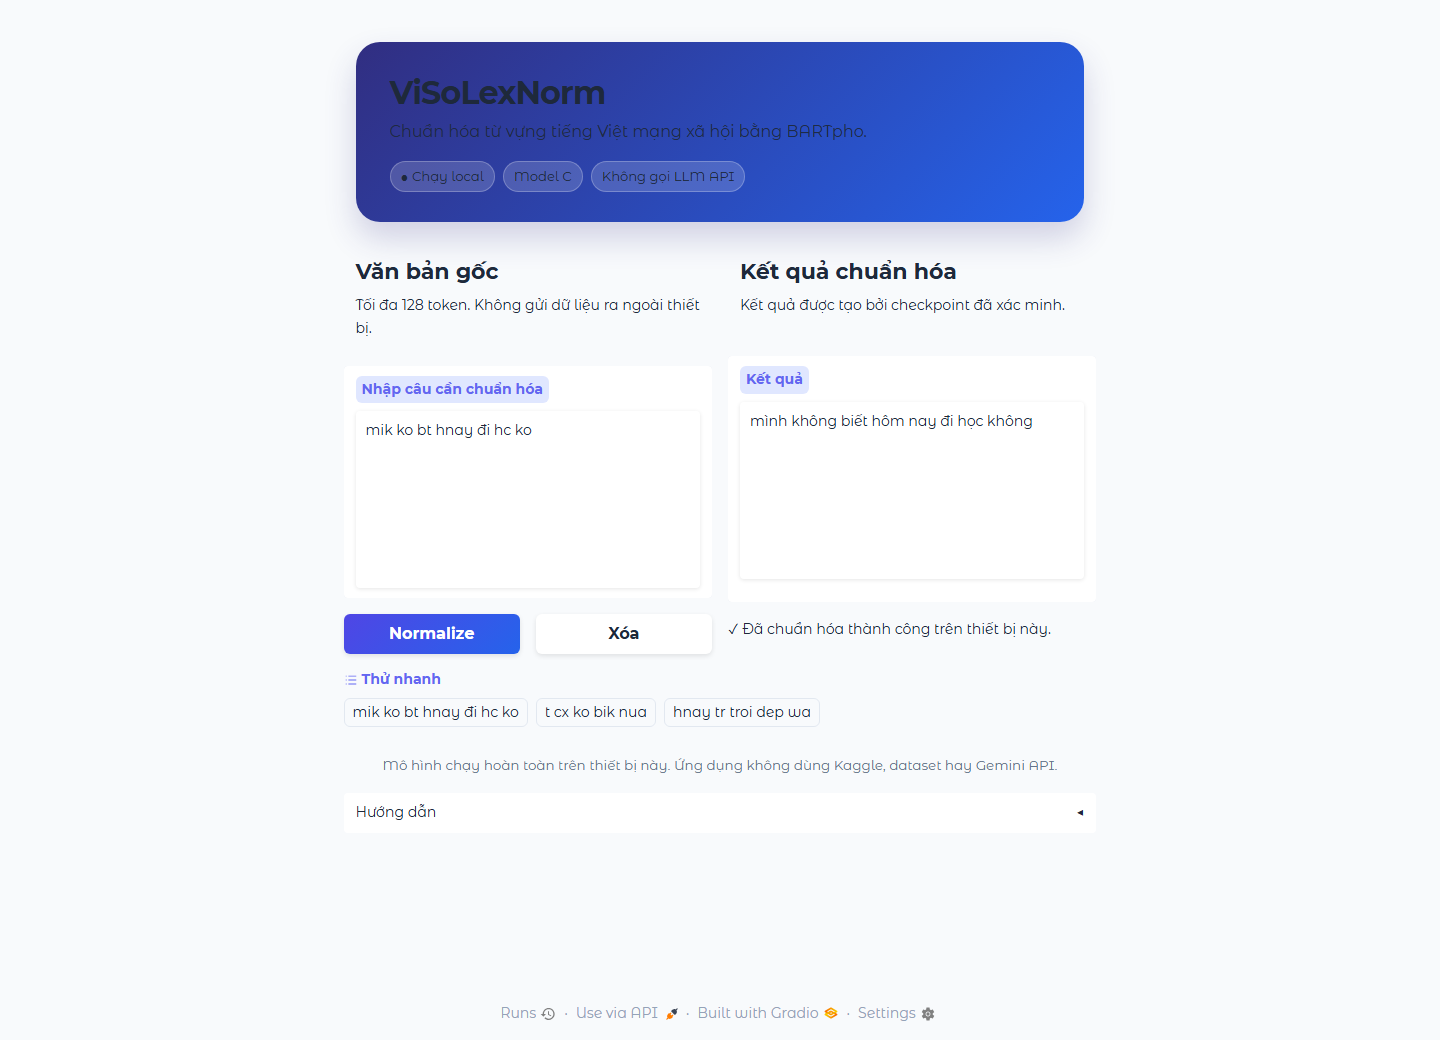
\includegraphics[width=0.9\linewidth]{figures/gradio_model_c.png}
\caption{Local Gradio application using the Dev-selected Model~C checkpoint. The displayed normalization runs locally without a Gemini API call.}
\label{fig:gradio-app}
\end{figure}

\section{Limitations}

The LLM-reviewed weak labels are not equivalent to human annotations and were not human-verified at full scale. Temperature 0, a fixed prompt, structured schema validation, and deterministic filters improve reproducibility and reduce identifiable problems, but they do not guarantee that every accepted target is semantically optimal. Some lexical variants are context-dependent, and the LLM reviewer may select a plausible target that differs from the preferred annotation in ViLexNorm-style evaluation.

The comparison also changes more than one factor at a time. Model~A begins from the public BARTpho checkpoint, whereas Models~B and C begin from Model~A. Model~B and Model~C further differ in the size of their weak-label pools and in their number of epochs. The observed differences should therefore be described as properties of the three complete training configurations, not as a causal estimate of weak-label count alone.

The edit-based metric implementation is a deterministic project scorer rather than an independently validated official ViLexNorm evaluator. In addition, the 128-token truncation limit and CPU model-loading time may affect long inputs and interactive deployment settings.

\section{Conclusion}

This study compared three BARTpho-syllable configurations for Vietnamese social media lexical normalization. Model~A used only human-annotated ViLexNorm data, Model~B added an initial pool of 18,970 LLM-reviewed weak labels, and Model~C used an expanded pool of 64,813 LLM-reviewed weak labels. The common Test evaluation produced F1 values of 0.718184, 0.742215, and 0.764993 and ERR values of 0.600250, 0.633111, and 0.664725 for Models~A, B, and C, respectively. The results are consistent with LLM-reviewed social-media examples providing useful additional training variation.

Model~C was selected using the common Dev evaluation and is used as the default local application checkpoint, while Model~B remains available as a fallback. It subsequently achieved the highest values in the common Test evaluation. Future work should expand human auditing of accepted weak labels and separate the effects of training duration, initialization, and weak-label coverage more directly.

\bibliographystyle{plainnat}
\bibliography{references}

\end{document}